El detector TRITIUM, al igual que el veto actiu del sistema de rejecció del fons radioactiu, consisteix en una cadena de tres elements. El plastic de centelleig, que generen fotons en l'espectre visible com a resposta a la detecció d'una partícula, ja siga un decaïment del triti a la mostra o un esdeveniment del fons radioactiu. Els photosensors, que detecten aquests fotons visibles i, com a conseqüència, generen un pols electrònic. L'electrónica, encarregada de processar i analitzar aquests polsos electrònic. A la Figura \ref{fig:EsquemaDetector} es pot veure un esquema del detector descrit.

\begin{figure}[hbtp]
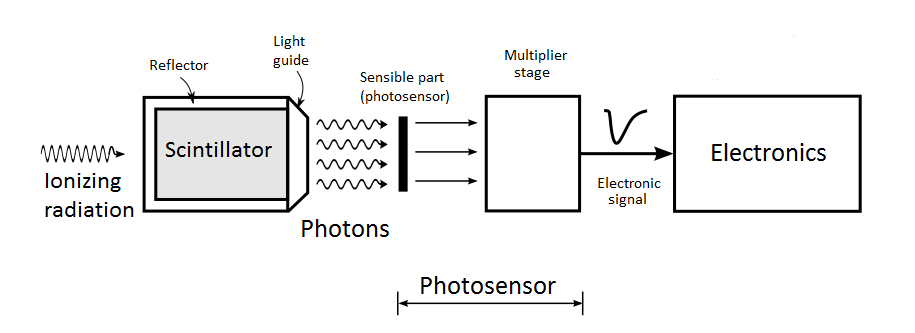
\includegraphics[scale=0.6]{12Summary/3DesignPrinciples/32Tritium_detector/ScintillatorDetector.png}
\centering
\caption{Esquema d'un detector de centelleig.\label{fig:EsquemaDetector}}
\end{figure}